\documentclass{ctexart}
\usepackage{amsmath}
\usepackage{booktabs}
\usepackage{newfloat}
\usepackage{graphicx}
\usepackage{minted}
\usepackage{booktabs, longtable}

\usepackage{minted}
\usemintedstyle{one-dark}
\setmonofont{Fira Code}
\newmintinline[mono]{python}{breakanywhere,fontsize=\small}
\newminted{python}{breakanywhere,tabsize=2,autogobble,breaklines=true,escapeinside=||,fontsize=\small}
\newenvironment{monos}{\VerbatimEnvironment\begin{pythoncode}}{\end{pythoncode}}

\usepackage{tikz}
\usepackage{pgfplots}
\pgfplotsset{compat=1.18}
\usetikzlibrary{external}
\tikzexternalize

\begin{document}
\section{数据集常见存储方式}

\begin{itemize}
    \item 文件名或者文件夹本身包含标注数据的信息。
    \item 一个专门的索引文件(如一个 CSV 表格),用于标注数据。
\end{itemize}

对于基因和生物组数据,我们可能使用二进制数据库或者网络流来存储这些数据。但是,但多数常
见的数据集都是以上述方式存储的。

\begin{monos}
from fastai.vision.all import *
path = untar_data(URLs.PETS)
path.ls()
#[Path('/root/.fastai/data/oxford-iiit-pet/images'),Path('/root/.fastai/data/oxford-iiit-pet/annotations')]
\end{monos}

我们发现,提供了两个文件夹,一个是图像,一个是标注。

\begin{monos}
(path / "images").ls()
#(#7393) [Path('/root/.fastai/data/oxford-iiit-pet/images/Siamese_87.jpg'),
\end{monos}

对于图像文件夹中,使用 \mono!ls! 返回了一个 \mono!L! 类型的集合。该集合是 \mono!fastai!
所特有的,打印时会显示自己的长度、部分元素(过多部分会被省略)。

这些宠物文件名的格式可以以如下 \mono!Regex! 表示: \\
\verb!/^(?P<breed_name>[A-Za-z_]+)_(?P<number>\d+)\.jpg$/! 借此,我们可以得到宠物的种
类和编号。

\begin{monos}
fname = (path / "images").ls()[0]
next(re.finditer(r'(?P<breed_name>[A-Za-z_]+)_(?P<number>\d+)\.jpg$', fname.name)).groupdict() #Deal with Latex Workshop's Parser$
# {'breed_name': 'Siamese', 'number': '87'}
\end{monos}

\begin{monos}
pets = DataBlock(
    blocks=(ImageBlock, CategoryBlock),
    get_items=get_image_files,
    splitter=RandomSplitter(seed=42),
    get_y=lambda path: re.search(
        r"(?P<breed_name>[A-Za-z0-9_]+)_(?P<number>\d+)\.jpg$", path.name
    ).group(
        "breed_name"
    ),  #$ Apply labeling to path's name. Equiv: using_attr(RegexLabller(regex), 'name') since RegexLabeller use group 1 by default.shi hou
    item_tfms=Resize(460),
    batch_tfms=aug_transforms(size=224, min_scale=0.75),
)
dls = pets.dataloaders(path / 'images')
\end{monos}

我们创建 \mono!DataBlock! 对象来创建 \mono!DataLoader! 对象。特别的,我们没有直接把所有
的照片都变成 244 大小,而是先将他们随机裁剪成 460 大小,然后再将其缩放到 224 大小。 这
样做可以避免在 \mono!aug_transforms! 时,大量的像素被 interpolated, 产生质量低的数据。

简言之,我们采用这样的策略:

\begin{itemize}
    \item 首先将图片缩放到大于目标尺寸两倍或以上的大小
    \item 然后将所有的 data augmentation, pixel interpolation 的操作一并使用 GPU 完成,
          而非对每张图片单独进行。这样,更多的 data augmentation 可以运行而不至于造成大量的
          empty zones。减少的 interpolation 保证了数据的质量。
\end{itemize}

\begin{figure}[H]
    \centering
    \includegraphics[width=0.8\textwidth]{assets/interpolation_example.png}
    \caption{Interpolation example}
\end{figure}

实现这个过程只需要加入 \mono!Resize! 并在 \mono!aug_functions! 中添加 \\
\mono!min_size!即可 (自动的 \mono!RandomResizeCrop!)。传统的 AI 库将会更多次
interpolate 图像,从而产生质量很低的数据。

为了避免错误的数据,我们应当在训练前检查数据——确保一切正常。鉴于我们往往在一些不熟悉的
领域工作,Google 来保证这些图片以及其标注都是正确的。

\begin{monos}
dls.show_batch(nrows=1, max_n=4)
\end{monos}

\begin{figure}[H]
    \centering
    \includegraphics[width=0.8\textwidth]{assets/pets_batch.png}
    \caption{Pets batch}
\end{figure}

如果展示的数据看起来不对劲,可以使用 \mono!summary! 让 \mono!fastai! 打印出生成一个数据
时每一步的信息,以及在什么地方出现了错误,等等。

\section{训练一个基线}

当数据看起来没有问题的时候,训练一个简单的模型作为基准线。这帮助我们认识到有没有必要收
集更多的数据,学习并使用大量的 domain specific 工程技术,并且建立一个对最终模型心理预
期。

\begin{monos}
learn = vision_learner(dls, resnet34, metrics=accuracy)
learn.fine_tune(2)
\end{monos}

让模型学习一次所有数据(one complete pass through all the data),就是一个 epoch。

\subsection{cross entropy loss}

fastai 在这里选择 cross entropy loss,作为默认的损失函数,因为它

\begin{itemize}
    \item 可以处理存在两个及以上因变量的情况
    \item 更快,更可靠的训练
\end{itemize}

\subsubsection{理解 cross entropy loss}

获得一个 mini-batch。我们定义了 mini-batch 的大小为 64。

\begin{monos}
x, y = dls.one_batch()
preds, trgts = learn.get_preds(dl=[(x, y)])
preds.shape, trgts.shape
# (torch.Size([64, 37]), torch.Size([64]))
\end{monos}

上面的 \mono!trgts == y!,所以实际上可以被忽略。预计的结果是一个长度为 37 的 tensor,也
就是表示 37 个不同宠物类型的概率 —— 他们和为 1。为了保证这一点,我们需要使用
\mono!softmax! 函数。

\subsubsection{Softmax}

我们使用这个激活函数来保证所有的 activations 都在 0 到 1 之间,并且他们的和也是 1。这个
函数类似于 sigmoid 函数。 signmoid 函数看起来像这样:

\begin{equation}
    \sigma(x) = \frac{1}{1 + e^{-x}}
\end{equation}

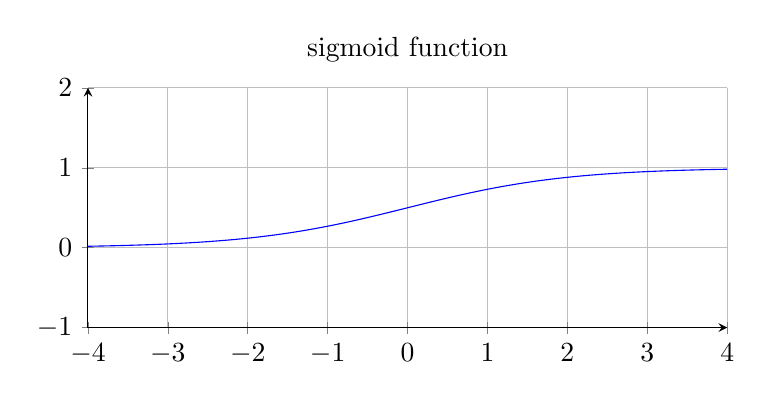
\begin{tikzpicture}
    \begin{axis}[
            title = {sigmoid function},
            grid = major,
            ymin = -1, ymax = 2,
            ytick = {-1, ..., 2},
            xtick = {-4, ..., 4},
            axis lines=left,
            axis equal image,
            width = 0.8\textwidth,
        ]
        \addplot[
            blue,
            domain = -4:4,
            samples = 100
        ]
        {1/(1+exp(-x))};
    \end{axis}
\end{tikzpicture}

sigmoid 函数只能处理一个 category 的情况 (binary classification problem) 。但是
softmax 函数可以处理更多的类别,并保证他们的和为 1,每个都大于 0,并且任何预测之间的区别
都将被指数级的放大。

\begin{monos}
acts = torch.randn((6, 2)) * 2 # prediction of 6 images of prob being 3/7
(acts[:, 0] - acts[:, 1]).sigmoid() # relative confidence

def softmax(x): 
    """
    Generialization of two column situation
    """
    return torch.exp(x) / torch.exp(x).sum(dim = 1, keepdim = True)

sm_acts = torch.softmax(acts, dim = 1)
\end{monos}


\begin{equation}
    \mathrm{softmax}(x) = \frac{e^{x_i}}{\sum_{j}e^{x_j}}
\end{equation}

\subsubsection{Log Likelihood 损失函数}

通过 softmax 函数,我们处理了损失函数的的第一部分。现在,我们希望让损失函数处理更多类型
的输入。

\begin{monos}
target = torch.randint(0, 2, (6,))
idx = torch.arange(6)
sm_acts = torch.softmax(acts, dim = 1)
sm_act[idx, target] # 得到是 target 的可能性。对于 n 个不同的 category, 得到的都是这个模型预计的是结果为 target 的概率。
\end{monos}

\mono!PyTorch! 提供了这个函数的实现。

\begin{monos}
F.nil_loss(sm_acts, targ, reduction = 'none')
\end{monos}

这里,如果 reduction = 'none',那么返回一个 tensor,否则返回一个 scalar(平均值)。这里
的,NIL 表示 negative log likelihood。

使用这个函数之后,我们应该计算 \mono!torch.log!——我们希望让这些 0 到 1 之间的概率转化为
负无穷到无穷之间。我们将每个概率进行对数运算,然后求其平均,得到 negative log
likelihood loss。PyTorch 的 softmax 假设你已经计算了 log, 所以不会给我们计算 log。

首先计算 softmax, 然后求 log,得到的就是 cross entropy loss。这个函数有 \\
\mono!nn.CrossEntropyLoss! 以及 \mono!F.cross_entropy! 两个实现。他首先计算 \mono!log_softmax!,然后计算 \mono!nil_loss!。

\begin{monos}
loss_func = nn.CrossEntropyLoss()
loss = loss_func(acts, target)
# OR
loss = F.cross_entropy(acts, target)
\end{monos}

使用 \mono!reduction='none'! 来避免计算平均值。

\subsection{Model Interpretion}

\begin{monos}
interp = ClassificationInterpretation.from_learner(learn)
interp.plot_confusion_matrix()
\end{monos}

然后我们就获得了一个几乎无法阅读的巨大矩阵。因此,我们使用
\mono!most_cofused(min_val=5)! (有至少 5 个错误的预测),来尝试理解这个模型。

\begin{monos}
interp.most_confused(min_val=5)
\end{monos}

结果告诉我们,这些被错误的预测的图像连专家有时都没能达成一致意见。

\subsection{Improve Model}

选择一个更好的的 learE\textbf{}ning rate。

\subsubsection{Learning Rate Finder}

我们刚开始没有定义 learning rate,因为 fastai 默认为我们定义 lr = 2.0e-3。

让我们尝试 0.1 作为 learning rate。这样做反而降低了准确率,因为 lr 太大,优化器走出了过
大的一步,以至于模型没能收敛。

解决方案:

\begin{enumerate}
    \item 首先选择一个极小的 learning rate。
    \item 使用这个 lr,对模型进行一个 mini-batch 的训练。
    \item 如果模型的 loss 有所进步,我们就将 lr 变成 lr * 2;反之,就停下。
\end{enumerate}

使用这个算法,我们可以得到一个比较好的 learning rate——一般为最后一轮 lr / 10 或者直接是
最后一轮的 lr。

\begin{monos}
learn = cnn_learner(dls, resnet34, metrics=accuracy)
lr_min, lr_steep = learn.lr_find() # min / 10: 8.32e-03, steepest: 6.31e-03
# 从图像可知,比较合适的 learning rate 为 3e-3
\end{monos}

\begin{figure}[H]
    \centering
    \includegraphics[width=0.8\textwidth]{assets/lr_finder.png}
    \caption{Learning rate finder}
    \label{fig:lr_finder}
\end{figure}

\subsubsection{Transfer Learning}

我们的模型利用了一个已经训练好的模型——这些模型经过大量数据的洗礼,整体上精通于图像分类
方面的任务。我们前面那些层中已经识别出的特征(如眼球,边缘,形状,等等),并把最后一层
替换为完全随机的一层作为我们的新层。

我们希望避免前面那些层的参数被破坏——所以,我们让 optimizer 只更新最后一层的参数。这被称
为 freezing pretrained layers。默认的行为是这样的:

\begin{itemize}
    \item freeze pretrained layers,训练一轮
    \item 然后解冻所有层,训练要求的轮数
\end{itemize}

\begin{table}[H]
    \begin{longtable}[]{@{}lllll@{}}
        \toprule()
        epoch & train\_loss & valid\_loss & accuracy & time  \\
        \midrule()
        \endhead
        0     & 1.341070    & 0.348429    & 0.888363 & 02:07 \\
        \bottomrule()
    \end{longtable}

    \begin{longtable}[]{@{}lllll@{}}
        \toprule()
        epoch & train\_loss & valid\_loss & accuracy & time  \\
        \midrule()
        \endhead
        0     & 0.533813    & 0.416962    & 0.882273 & 02:08 \\
        1     & 0.327838    & 0.242440    & 0.925575 & 02:09 \\
        \bottomrule()
    \end{longtable}
    \caption{Default Behavior}
    \label{fig:default_learner}
\end{table}

但是我们可以做的更好:让我们直接使用 \mono!fit_one_cycle! 手工完成这个过程。

我们解冻之后,应当对每一层采用不同的 learning rate (discriminative learning rate):前面
的那些层的 learning rate 已经被无限次的训练过,并且往往对任何图像分类的工作都是有意义
的。因此,前面的那些层应当采用更小的 learning rate,而我们附加的随即层应当使用更高的
learning rate。

因此,我们传入一个元组,分别表示最大和最小的 learning rate 来进行训练。

\begin{monos}
learn = vision_learner(dls, resnet34, metrics=accuracy)
# Train randomly added layers for 3 epoches.
# fit_one_cycle 从很小的 lr 开始,增加 lr, 最后再减少
learn.fit_one_cycle(3, 3e-3)
learn.unfreeze()
# 因为层数增加了,所以需要再次寻找 learning rate
# 因为模型已经被训练了,所以我们直接使用平坦区域的中间部分即可(不会出现 loss 减少,很正常)
learn.lr_find()
# 返回一个建议,SuggestedLRs(valley=0.00010964782268274575)
learn.fit_one_cycle(12, lr_max=slice(1e-6, 1e-4))
\end{monos}

\begin{figure}[H]
    \centering
    \includegraphics[width=0.8\textwidth]{assets/lr_unfreeze.png}
    \caption{Unfreezed and Learning Rate}
    \label{fig:lr_unfreeze}
\end{figure}


\begin{longtable}[]{@{}lllll@{}}
    \toprule()
    epoch & train\_loss & valid\_loss & accuracy & time  \\
    \midrule()
    \endhead
    0     & 1.174035    & 0.343256    & 0.887010 & 02:08 \\
    1     & 0.518981    & 0.264255    & 0.913396 & 02:07 \\
    2     & 0.327522    & 0.223678    & 0.928281 & 02:07 \\
    \bottomrule()
\end{longtable}

\begin{longtable}[]{@{}lllll@{}}
    \toprule()
    epoch & train\_loss & valid\_loss & accuracy & time  \\
    \midrule()
    \endhead
    0     & 0.276333    & 0.212369    & 0.932341 & 02:09 \\
    1     & 0.252017    & 0.197693    & 0.938430 & 02:09 \\
    2     & 0.225424    & 0.198766    & 0.943166 & 02:09 \\
    3     & 0.211397    & 0.202609    & 0.936401 & 02:09 \\
    4     & 0.192819    & 0.192085    & 0.942490 & 02:10 \\
    5     & 0.176632    & 0.192738    & 0.942490 & 02:09 \\
    6     & 0.165869    & 0.191011    & 0.939784 & 02:09 \\
    7     & 0.133440    & 0.181678    & 0.945196 & 02:09 \\
    8     & 0.135830    & 0.181335    & 0.947226 & 02:08 \\
    9     & 0.130303    & 0.179268    & 0.947226 & 02:09 \\
    10    & 0.125759    & 0.184461    & 0.945196 & 02:08 \\
    11    & 0.122549    & 0.181916    & 0.944520 & 02:09 \\
    \bottomrule()
\end{longtable}


And we overfitted.


\begin{monos}
learn.recorder.plot_loss()
\end{monos}

\begin{figure}[H]
    \centering
    \includegraphics[width=0.8\textwidth]{assets/train_loss.png}
    \caption{Loss of Training and Validation}
    \label{fig:loss}
\end{figure}

我们发现,validation set 的 loss 竟然保持不变了。这不是什么大问题,因为我们的 metrics
(accuracy)一直在提升,loss 不过是计算机使用的。我们在实践中,只关心模型的 metrics 的
变化 —— loss 会比 accuracy 更先一步停止提升,因为模型开始对数据 overconfident。在过一段
时间,metrics 会停止提升,因为模型开始背诵数据集。

在此之前,模型在每个 epoch 都被保存一次,然后寻找具有最好 accuracy 的模型 —— early
stopping。 但是这不是个好主意,因为 learning rate 在中间往往很低,个模型一个过拟合的机
会。因此,如果我们发现产生了过拟合,应当调整 epochs 然后重新训练。

\subsection{Export}

\mono!lambda! 函数无法被导出,所以必须使用命名函数。



\subsubsection{TPU}

更深层次的训练模型往往(不总是)能够提供更好的结果(对数据进行更好的拟合)。但是,这也
意味着需要更多的 GPU 内存,更小的 batch size (\mono!DataBlock(bs = x)! 来修改) 来避免
OOM,以及更长的训练时间。

为了加速这个过程,可以使用 float 16 而非 double 来进行训练。

\begin{monos}
from fastai.callbacks.fp16 import *
learn = vision_learner(dls, resnet34, metrics=accuracy).to_fp16()
learn.fit_one_cycle(3, 3e-3)
\end{monos}

上述代码使用 fp16 来加速训练。

\end{document}
